%%%%%%%%%%%%%%%%%%%%%%%%%%%%%%%%%%%%%%%%%%%%%%%%%%%%%%%%%%%%%%%%%%%%%%%%%%%%%%%%
%%%%%%%%%%%%%%%%%%%%%%%%%%%%%%%%%%%%%%%%%%%%%%%%%%%%%%%%%%%%%%%%%%%%%%%%%%%%%%%%
%
% A general frame for lecture slides and lecture notes in one file
% using LaTeX beamer
%
%%%%%%%%%%%%%%%%%%%%%%%%%%%%%%%%%%%%%%%%%%%%%%%%%%%%%%%%%%%%%%%%%%%%%%%%%%%%%%%%
%%%%%%%%%%%%%%%%%%%%%%%%%%%%%%%%%%%%%%%%%%%%%%%%%%%%%%%%%%%%%%%%%%%%%%%%%%%%%%%%
\documentclass[aspectratio=169,11pt]{beamer}
%\usepackage[ngerman]{babel}
\usepackage[T1]{fontenc}
\usepackage[utf8]{inputenc}
\usepackage{amsmath,amssymb,amsfonts}


% only presentation
\mode<presentation>
{
  \usepackage[course]{dunestyle-beamer}
}

% all after
\usepackage{amscd}

\usepackage{pgfplots,adjustbox}
\usepackage{eurosym}
\usepackage{graphicx}
\graphicspath{{.}{figures/}{../../latexstyle/layout/}}
%\usepackage{picinpar}
%\usepackage{fancybox}
%\usepackage{xspace}
\usepackage{enumerate}
\usepackage{algpseudocode}
\usepackage{color}
\usepackage{bold-extra}
\usepackage{bm}
\usepackage{stmaryrd}
%\usepackage[squaren]{SIunits}
\usepackage{nicefrac}

\usepackage{fancyvrb,bbm,xspace}
\usepackage{lmodern}
\usepackage{fancyvrb,bbm,xspace}
\usepackage[binary-units]{siunitx}
\usepackage{xcolor,tabu}

\usepackage{lmodern}
\usepackage{inconsolata}
\usepackage{nimbusmononarrow}
%\renewcommand*\ttdefault{txtt}
\usepackage{dsfont}

\mode<presentation>
{
\theoremstyle{definition}
}
\newtheorem{Def}{Definition}%[section]
\newtheorem{Exm}[Def]{Example}
\newtheorem{Lem}[Def]{Lemma}
\newtheorem{Rem}[Def]{Remark}
\newtheorem{Rul}[Def]{Rule}
\newtheorem{Thm}[Def]{Theorem}
\newtheorem{Cor}[Def]{Corollary}
\newtheorem{Obs}[Def]{Observation}
\newtheorem{Ass}[Def]{Assumption}
\newtheorem{Pro}[Def]{Property}
\newtheorem{Alg}[Def]{Algorithm}
\newtheorem{Prp}[Def]{Proposition}
\newtheorem{Lst}[Def]{Listing}

% Delete this, if you do not want the table of contents to pop up at
% the beginning of each subsection:
\AtBeginSection[]
{
  \begin{frame}<beamer>
    \frametitle{Contents}
    \tableofcontents[sectionstyle=show/shaded,subsectionstyle=hide/hide/hide]
%\tableofcontents[currentsection]
  \end{frame}
}

% Title definition
\title{DUNE PDELab Tutorial 01}
\subtitle{Conforming FEM for a Nonlinear Poisson Equation}
\author{Peter Bastian}
\institute[]
{
  IWR\\
  Heidelberg University
}

%%%%%%%%%%%%%%%%%%%%%%%%%%%%%%%%%%%%%%%%%%%%%%%%%%%%%%%%%%%%%%%%%%%%%%%%%%%%%%%%
%%%%%%%%%%%%%%%%%%%%%%%%%%%%%%%%%%%%%%%%%%%%%%%%%%%%%%%%%%%%%%%%%%%%%%%%%%%%%%%%
%
% now comes the individual stuff lecture by lecture
%
%%%%%%%%%%%%%%%%%%%%%%%%%%%%%%%%%%%%%%%%%%%%%%%%%%%%%%%%%%%%%%%%%%%%%%%%%%%%%%%%
%%%%%%%%%%%%%%%%%%%%%%%%%%%%%%%%%%%%%%%%%%%%%%%%%%%%%%%%%%%%%%%%%%%%%%%%%%%%%%%%

\begin{document}

\frame[plain, noframenumbering]{\titlepage}

%%%%%%%%%%%%%%%%%%%%%%%%%%%%%%%%%%%%%%%%%%%%%%%%%%%%%%%%%%%%%%%%%%%%%%%%%%%%%%%%
%%%%%%%%%%%%%%%%%%%%%%%%%%%%%%%%%%%%%%%%%%%%%%%%%%%%%%%%%%%%%%%%%%%%%%%%%%%%%%%%

\begin{frame}
\frametitle{Motivation}
This tutorial extends on tutorial 00 by
\begin{enumerate}[1)]
\item Solving a \textbf{nonlinear} stationary PDE
\item Using conforming finite element spaces of \textbf{arbitrary order}
\item Using \textbf{different types of (conforming) meshes} (simplicial and cubed)
\item Using \textbf{different types of boundary conditions}
\end{enumerate}
\end{frame}

\begin{frame}
\frametitle{PDE Problem}
We consider the problem
\begin{subequations} \label{eq:ProblemStrong}
\begin{align}
-\Delta u + q(u) &= f &&\text{in $\Omega$},\\
u &= g &&\text{on $\Gamma_D\subseteq\partial\Omega$},\\
-\nabla u\cdot \nu &= j &&\text{on $\Gamma_N=\partial\Omega\setminus\Gamma_D$}.
\end{align}
\end{subequations}
\begin{itemize}
\item $q:\mathbb{R}\to\mathbb{R}$ a nonlinear function
\item $f: \Omega\to\mathbb{R}$ the source term
\item $g: \Omega\to\mathbb{R}$ a function for Dirichlet boundary conditions on $\Gamma_D$
\item $j : \Gamma_N\to\mathbb{R}$ a function for Neumann (flux) boundary conditions
\item $\nu$: unit outer normal to the domain
\end{itemize}
\end{frame}

\begin{frame}
\frametitle{Weak Formulation}
now reads as follows:
\begin{equation}
\text{Find $u\in U$ s.t.:} \quad r^{\text{NLP}}(u,v)=0 \quad \forall v\in V,
\label{Eq:BasicBuildingBlock}
\end{equation}
with the continuous residual form
\begin{equation*}
r^{\text{NLP}}(u,v) = \int_\Omega \nabla u \cdot \nabla v + (q(u)-f)v\,dx + \int_{\Gamma_N} jv\,ds
\label{eq:ResidualForm}
\end{equation*}
and the function spaces
\begin{itemize}
\item $U= \{v\in H^1(\Omega) \,:\, \text{``$v=g$'' on $\Gamma_D$}\}$ (affine space)
\item $V= \{v\in H^1(\Omega) \,:\, \text{``$v=0$'' on $\Gamma_D$}\}$
\end{itemize}
\medskip
We \textbf{assume} that this problem has a unique solution
\end{frame}

\begin{frame}
\frametitle{Algebraic Problem}
\rightarrownice Solve weak formulation in finite-dimensional setting
\begin{equation*}
U_h=\text{span}\{\phi_1,\ldots,\phi_n\} + u_{h,g}, \quad V_h=\text{span}\{\psi_1,\ldots,\psi_n\}
\end{equation*}

Expanding $u_h=u_{h,g} + \sum_{j=1}^n (z)_j\phi_j$
results in an algebraic equation for $z\in\mathbb{R}^n$:
\begin{align*}
\text{Find $u_h\in U_h$ s.t.:} && r(u_h,v)&=0 && \forall v\in V_h\\
\Leftrightarrow{} && r\left(u_{h,g} +\sum_{j=1}^n (z)_j\phi_j,\psi_i\right) &= 0 &&\forall i=1,\ldots,n\\
\Leftrightarrow{} && R(z) = 0,
\end{align*}
with $R: \mathbb{R}^n \to \mathbb{R}^n$ and $R_i(z) = R\left(u_{h,g} +\sum_{j=1}^n (z)_j\phi_j,\psi_i\right)$ \\
\medskip
\textbf{Note:} We remark on the realization of Dirichlet conditions below
\end{frame}

\begin{frame}
\frametitle{Solution of Algebraic Problem}
Use {\em iterative} methods to solve $R(z)=0$. Fixed point iteration reads:
\begin{equation}
z^{(k+1)} = G(z^{(k)}) = z^{(k)} - \lambda^{k} W(z^{(k)}) R(z^{(k)}) .
\end{equation}
\vspace{-5mm}
\begin{itemize}
\item $\lambda^{k}\in\mathbb{R}$ is a damping factor
\item $W(z^{(k)})$ is a preconditioner matrix, e.g. in Newton's method one uses
\begin{equation*}
W(z^{(k)}) = (J(z^{(k)}))^{-1} \quad \text{where $(J(z^{(k)}))_{i,j} = \frac{\partial R_i}{\partial z_j}
(z^{(k)})$}
\end{equation*}
i.e. one needs to solve $J\left(z^{(k)}\right) w = R(z^{(k)})$ per iteration
\end{itemize}
The following algorithmic building blocks are required:
\begin{enumerate}[i)]
\item residual evaluation $R(z)$,
\item Jacobian evaluation $J(z)$ (or an approximation of it),
\item alternatively: matrix-free Jacobian application $J(z) w$ (or an approximation).
\end{enumerate}
\end{frame}

\begin{frame}
\frametitle{Note on Matrix-free Evaluation}
\textbf{Nonlinear case:}
\begin{equation*}
(J(z) w)_i = \sum_{j=1}^n (J(z))_{i,j} (w)_j = \sum_{j=1}^n
\frac{\partial}{\partial z_j} r\left(u_{h,g}+\sum_{l=1}^n (z)_l  \phi_l,\psi_i\right) (w)_j .
\end{equation*}
\textbf{Linear case:} $r(u,v)=a(u,v)-l(v)$, $a$ BLF, $l$ LF
\begin{equation*}
\begin{split}
(J(z) w)_i &= \sum_{j=1}^n
\frac{\partial}{\partial z_j} r\left(u_{h,g}+\sum_{l=1}^n (z)_l  \phi_l,\psi_i\right) (w)_j \\
&= \sum_{j=1}^n \frac{\partial}{\partial z_j} \left(
a\left(u_{h,g}+\sum_{l=1}^n (z)_l  \phi_l,\psi_i\right) - l(\psi_i)\right) (w)_j \\
&= \sum_{j=1}^n \frac{\partial}{\partial z_j} \left(
\sum_{l=1}^n (z)_l a(\phi_l,\psi_i) \right)  (w)_j 
= \sum_{j=1}^n a(\phi_j,\psi_i) (w)_j =
a\left( \sum_{j=1}^n (w)_j \phi_j,\psi_i\right) \\
&= (A w)_i
\end{split}
\end{equation*}
\end{frame}

\begin{frame}
\frametitle{Recall Finite Element Mesh Notation}
\begin{enumerate}[i)]
\item Ordered sets of vertices and elements:
$$\mathcal{X}_h = \{x_1,\ldots,x_N\}, \quad\mathcal{T}_h = \{T_1, \ldots, T_M\}$$
\item Partitioning of vertex index set $\mathcal{I}_h=\{1,\ldots,N\}$ into $
\mathcal{I}_h = \mathcal{I}_h^{int}\cup\mathcal{I}_h^{\partial\Omega}$:
\begin{equation*}
\mathcal{I}_h^{int} = \{i\in \mathcal{I}_h\,:\, x_i\in\Omega\},
\quad \mathcal{I}_h^{\partial\Omega} = \{i\in \mathcal{I}_h\,:\, x_i\in\partial\Omega\}.
\end{equation*}
\item For every element $T\in\mathcal{T}_h$ a local-to-global map
$$g_T:\{0,\ldots,n_T-1\}\to\mathcal{I}_h$$
\item For every element $T\in\mathcal{T}_h$ an element transformation map
$$\mu_T : \hat T \to T$$
$\mu_T$ is differentiable with invertible Jacobian and consistent with $g_T$:
$$\forall i\in\{0,\ldots,n_T-1\} : \mu_T(\hat x_i) = x_{g_T(i)}$$
\end{enumerate}
\end{frame}

\begin{frame}
\frametitle{Conforming Finite Element Space}
with \textbf{polynomial degree} $k$ in \textbf{dimension} $d$ on \textbf{mesh} $\mathcal{T}_h$:
\begin{equation*}
V_h^{k,d}(\mathcal{T}_h) = \left\{ v\in C^0(\overline{\Omega}) \,:\,
\forall T\in\mathcal{T}_h : v|_T = \hat p_T \circ \mu_T^{-1} \wedge \hat p_T\in\mathbb{P}_T^{k,d}\right\}
\end{equation*}
where the multivariate polynomials $\mathbb{P}_T^{k,d}$ depend on element type:
{\small\begin{equation*}
\mathbb{P}_T^{k,d} = \left\{\begin{array}{ll}
\left\{ p\,:\, p(x_1,\ldots,x_d) = \sum\limits_{0\leq\|\alpha\|_1\leq k} c_\alpha
x_1^{\alpha_1}\cdot\ldots\cdot x_d^{\alpha_d}\right\} & \text{$\hat T = \hat S$ (simplex)}, \\
\left\{ p\,:\, p(x_1,\ldots,x_d) = \sum\limits_{0\leq\|\alpha\|_\infty\leq k} c_\alpha
x_1^{\alpha_1}\cdot\ldots\cdot x_d^{\alpha_d}\right\} & \text{$\hat T = \hat C$ (cube)}
\end{array}\right .
\end{equation*}}
The dimension of $\mathbb{P}^{k,d}_T$ is:
\begin{equation*}
n_{\hat C}^{k,d} = (k+1)^d \text{ (cube) },  \
n_{\hat S}^{k,d} = \left\{ \begin{array}{ll}
1 & k=0 \vee d=0\\
\sum\limits_{i=0}^k n_{\hat S}^{i,d-1} &\text{else}
\end{array}\right . \text{ (simplex) }
\end{equation*}
\end{frame}

\begin{frame}
\frametitle{Local Lagrange Basis}
\begin{center}
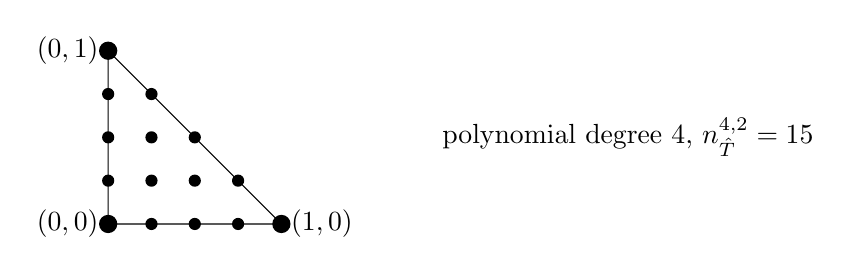
\begin{tikzpicture}[scale=1.1]
\draw (0,0) -- (2,0) -- (0,2) -- cycle;
%\draw[gray] (0.5,0.0) -- (2.0,1.5);
%\draw[gray] (1.0,0.0) -- (2.0,1.0);
%\draw[gray] (1.5,0.0) -- (2.0,0.5);
%\draw[gray] (0.5,0.5) -- (2.0,0.5);
%\draw[gray] (1,1) -- (2.0,1);
%\draw[gray] (1.5,1.5) -- (2.0,1.5);
%\draw[gray] (0.5,0.0) -- (0.5,0.5);
%\draw[gray] (1.0,0.0) -- (1.0,1.0);
%\draw[gray] (1.5,0.0) -- (1.5,1.5);
\node[left] at (0,0) {$(0,0)$};
\node[right] at (2,0) {$(1,0)$};
\node[left] at (0,2) {$(0,1)$};
\fill(0,0) circle (3pt);
\fill(2,0) circle (3pt);
\fill(0,2) circle (3pt);
\fill(0.5,0) circle (2pt);
\fill(1,0) circle (2pt);
\fill(1.5,0) circle (2pt);
\fill(0,0.5) circle (2pt);
\fill(0.5,0.5) circle (2pt);
\fill(1,0.5) circle (2pt);
\fill(1.5,0.5) circle (2pt);
\fill(0,1) circle (2pt);
\fill(0.5,1) circle (2pt);
\fill(1,1) circle (2pt);
\fill(0,1.5) circle (2pt);
\fill(0.5,1.5) circle (2pt);
\node at (6,1) {polynomial degree $4$, $n_{\hat T}^{4,2}=15$};
\end{tikzpicture}
\end{center}
Lagrange points and polynomials (shape functions) on $\hat T$:
$$L_{\hat T} = \left\{ \hat x^{\hat T}_0,\ldots,\hat x^{\hat T}_{n_{\hat T}^{k,d}-1} \right\}, \quad
P_{\hat T} = \left\{ \hat p^{\hat T}_0,\ldots,\hat p^{\hat T}_{n_{\hat T}^{k,d}-1}\right\}$$
such that $$\hat p^{\hat T}_i(\hat x^{\hat T}_j) = \delta_{i,j}$$
Extend local to global map:
\begin{equation*}
g_T : \{0,\ldots,n_{\hat T}^{k,d}-1\} \to \mathcal{I}_h^{k,d} =
\left\{0,\ldots,\text{dim} V_h^{k,d}(\mathcal{T}_h)-1\right\}
\end{equation*}
\end{frame}

\begin{frame}
\frametitle{Global Lagrange Basis}
\begin{center}
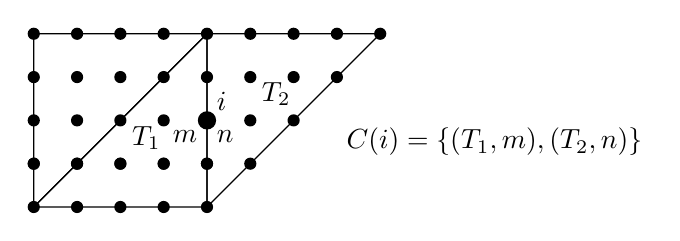
\begin{tikzpicture}[scale=1.1]
\draw (0,0) -- (2,0) -- (2,2) -- cycle;
\draw (0,0) -- (2,2) -- (0,2) -- cycle;
\draw (2,0) -- (2,2) -- (4,2) -- cycle;
\fill(0,0) circle (2pt);
\fill(2,0) circle (2pt);
\fill(2,2) circle (2pt);
\fill(0,2) circle (2pt);
\fill(4,2) circle (2pt);
\fill(1,0) circle (2pt);
\fill(0,1) circle (2pt);
\fill(1,1) circle (2pt);
\fill(2,1) circle (3pt);
\fill(3,1) circle (2pt);
\fill(1,2) circle (2pt);
\fill(3,2) circle (2pt);
\fill(0.5,0) circle (2pt);
\fill(1.5,0) circle (2pt);
\fill(0.0,0.5) circle (2pt);
\fill(0.5,0.5) circle (2pt);
\fill(1.0,0.5) circle (2pt);
\fill(1.5,0.5) circle (2pt);
\fill(2.0,0.5) circle (2pt);
\fill(0.0,0.5) circle (2pt);
\fill(0.5,0.5) circle (2pt);
\fill(1.0,0.5) circle (2pt);
\fill(1.5,0.5) circle (2pt);
\fill(2.0,0.5) circle (2pt);
\fill(0.5,1) circle (2pt);
\fill(1.5,1) circle (2pt);
\fill(0.0,1.5) circle (2pt);
\fill(0.5,1.5) circle (2pt);
\fill(1.0,1.5) circle (2pt);
\fill(1.5,1.5) circle (2pt);
\fill(2.0,1.5) circle (2pt);
\fill(0.5,2) circle (2pt);
\fill(1.5,2) circle (2pt);
\fill(2.5,0.5) circle (2pt);
\fill(2.5,1) circle (2pt);
\fill(2.5,1.5) circle (2pt);
\fill(3.0,1.5) circle (2pt);
\fill(3.5,1.5) circle (2pt);
\fill(2.5,2) circle (2pt);
\fill(3.5,2) circle (2pt);
\node[above right] at (2,1) {$i$};
\node at (1.3,0.8) {$T_1$};
\node at (2.8,1.3) {$T_2$};
\node[below left] at (2,1) {$m$};
\node[below right] at (2,1) {$n$};
\node[right] at (3.5,0.75) {$C(i)=\{(T_1,m), (T_2,n)\}$};
\end{tikzpicture}
\end{center}
Define inversion of the local-to-global map:
\begin{equation*}
C(i) = \{(T,m)\in\mathcal{T}_h\times\mathbb{N} \,:\, g_T(m)=i\}
\end{equation*}
then the global Lagrange basis functions are
\begin{equation*}
\phi_i(x) = \left\{\begin{array}{ll}
\hat p^{\hat T}_m(\mu_T^{-1}(x)) & x\in T \wedge g_T(m)=i \\
0 & \text{else}
\end{array}\right. , \quad i\in\mathcal{I}_h^{k,d}.
\end{equation*}
corresponding to the global Lagrange points
\begin{equation*}
\mathcal{X}_h^{k,d} = \left\{ x_i\in\overline{\Omega} \,:\,
x_i=\mu_T(\hat x^{\hat T}_{m})  \wedge g_T(m)=i \right\}
\end{equation*}
\end{frame}

\begin{frame}
\frametitle{Dirichlet Boundary Conditions I}
Indices of Lagrange points on the Dirichlet boundary are:
\begin{equation*}
\mathcal{I}_h^{D,k,d} =
\left\{ i\in\mathcal{I}_h^{k,d}  \,:\,
x_i\in\mathcal{X}_h^{k,d} \cap\Gamma_D
\right\} .
\end{equation*}
Then the test space with zero Dirichlet condition is:
\begin{equation*}
V_{h,0}^{k,d}(\mathcal{T}_{h}) = \left\{
v\in V_{h}^{k,d}(\mathcal{T}_{h}) \,:\, v(x_i) = 0
\quad \forall i\in\mathcal{I}_h^{D,k,d}
 \right\}
\end{equation*}
For the trial space choose any extension
\begin{equation*}
u_{h,g} = \sum_{i\in \mathcal{I}_h^{k,d}}
g(x_i) \phi_i, \qquad \text{so $u_{h,g}(x_i)=g(x_i) \ \forall i\in\mathcal{I}_h^{D,k,d}$}
\end{equation*}
Then the trial space is
\begin{equation*}
U_{h}^{k,d}(\mathcal{T}_{h}) = \left\{ u\in V_h^{k,d}(\mathcal{T}_h)
\,:\, u = u_{h,g} + w \wedge w\in V_{h,0}^{k,d}(\mathcal{T}_{h})\right\} = u_{h,g} + V_{h,0}^{k,d}(\mathcal{T}_{h})
\end{equation*}
\end{frame}

\begin{frame}
\frametitle{Dirichlet Boundary Conditions II}
There are different options to realize Dirichlet conditions in practice:
\begin{enumerate}
\item Elimination of all Dirichlet conditions from the algebraic systems, i.e.
\begin{equation*}
R: \mathbb{R}^{n_0} \to \mathbb{R}^{n_0}, \qquad 
n_0 = \dim\left( V_{h,0}^{k,d}(\mathcal{T}_{h}) \right), \qquad
R_i(z) = R\left(u_{h,g} +\sum_{j=1}^n (z)_j\phi_j,\psi_i\right)
\end{equation*}
\item Keep degrees of freedom at Dirichlet boundary in the algebraic system, i.e.
\begin{equation*}
R: \mathbb{R}^n \to \mathbb{R}^n, \qquad n = \dim\left( V_{h}^{k,d}(\mathcal{T}_{h}) \right)
\end{equation*}
with \textit{additional} equations
\begin{equation*}
z_i = g(x_i), \qquad \forall i\in\mathcal{I}_h^{D,k,d}
\end{equation*}
\textbf{This approach is used in PDELab}
\item Nitsche's method: Essential boundary conditions are \textit{not} built into the function space, instead certain terms are added to
the weak formulation
\end{enumerate}
\end{frame}

\begin{frame}
\frametitle{General Constraints}
Dirichlet boundary conditions are a special case of the following\\
\bigskip
\textbf{Task:} Given $V_h = \text{span}\left\{\phi_j \,:\, j\in J_h=\{1,\ldots,n\}\right\}$
construct a subspace $\tilde{V}_h\subseteq V_h$\\
\bigskip
This is how it is done in PDELab:
\begin{enumerate}[1)]
\item Assume $V_h=\text{span}\{\phi_i \,:\, i\in J_h\}$
\item Select a subset of indices $\tilde{J}_h\subset J_h$, $\dim(\tilde{J}_h)$ is the dimension of the subspace $\tilde V_h$
\item Set $\tilde{V}_h = \text{span}\left\{\tilde\phi_j \,:\, j\in \tilde{J}_h\right\}$,
where the new basis functions have the form
\begin{equation*}
\tilde\phi_j = \phi_j + \sum_{l\in J_h\setminus\tilde{J}_h} (B)_{j,l} \phi_l, \qquad \forall j\in \tilde{J}_h.
\end{equation*}
\end{enumerate}
Any such subspace is thus characterized by $C=(\tilde{J}_h,B)$\\
PDELab implements general constraints in this way, e.g. for so-called hanging nodes
\end{frame}

\begin{frame}
\frametitle{Element-wise Computations}
Now return to the evaluation of the residual form, which is element-wise
\begin{equation*}
r^{\text{NLP}}\left(u,v\right) =
\sum_{T\in\mathcal{T}_h} \alpha_T^V(u,v)
  + \sum_{T\in\mathcal{T}_h} \lambda_T^V(v)
 + \sum_{F\in\mathcal{F}_h^{\partial\Omega}}\lambda_F^B(v)
\end{equation*}
with
\begin{align*}
\alpha_T^V(u,v) &= \int_T \nabla u \cdot \nabla v + q(u) v \,dx, &
\lambda_T^V(v) &= - \int_T f v \,dx, & 
\lambda_F^B(v) &= \int_{F\cap\Gamma_N} j v\,ds
\end{align*}
$\mathcal{F}_h^{\partial\Omega}$: intersections of
elements with the domain boundary, i.e.
$$F=T_F^-\cap\partial\Omega$$
with $T_F^-\in\mathcal{T}_h$ the ``minus'' element associated with $F$ (see tutorial 2)
\end{frame}

\begin{frame}
\frametitle{$\lambda$ Volume Term}
For any $(T,m)\in C(i)$ we obtain
\begin{equation*}
\begin{split}
\lambda_T^V(\phi_i) &= - \int_T f \phi_i \,dx =
- \int_{\hat T} f(\mu_T(\hat x)) \hat p_m^{\hat T}(\hat x) |\text{det} J_{\mu_T}(\hat x)|\, d\hat x .
\end{split}
\end{equation*}
$J_{\mu_T}$ is the Jacobian of the element map $\mu_T$\\
\medskip
This integral is computed using numerical quadrature\\
\medskip
Collect all contributions of $T$ in a small vector:
\begin{equation*}
(\mathcal{L}_T^V)_m = - \int_{\hat T} f(\mu_T(\hat x)) \hat p_m^{\hat T}(\hat x)
|\text{det} J_{\mu_T}(\hat x)|\, d\hat x.
\end{equation*}
\end{frame}

\begin{frame}
\frametitle{$\lambda$ Boundary Term}
For $F\in\mathcal{F}_h^{\partial\Omega}$ with $F\subseteq\Gamma_N$
and $(T_F^-,m)\in C(i)$ we obtain
\begin{equation*}
\begin{split}
\lambda_T^B(\phi_i) &= \int_{F} j v\,ds =
\int_{\hat F} j(\mu_F(\hat x)) \hat p_m^{\hat T}(\eta_F(\hat x))
\sqrt{|\text{det} (J^T_{\mu_F}(\hat x)J_{\mu_F}(\hat x))|} \,ds
\end{split}
\end{equation*}
The integration is more involved here because it is over a face:
\begin{itemize}
\item $\mu_F: \hat F \to F$ maps the reference element of the face to the face
\item $\eta_F: \hat F \to \hat T_F^-$ maps reference
element of the face to the reference element of $T_F^-$
\end{itemize}
Collect all contributions of $F$ in a small vector:
\begin{equation*}
(\mathcal{L}_T^B)_m =
\int_{\hat F} j(\mu_F(\hat x)) \hat p_m^{\hat T}(\eta_F(\hat x))
\sqrt{|\text{det} J^T_{\mu_T}(\hat x)J_{\mu_T}(\hat x)|} \,ds .
\end{equation*}
Numerical quadrature is applied to compute the integral
\end{frame}

\begin{frame}
\frametitle{$\alpha$ Volume Term}
For any $(T,m)\in C(i)$ we get
\begin{equation*}
\begin{split}
\alpha_T^V(u_h,\phi_i) &= \int_T \nabla u \cdot \nabla \phi_i + q(u) \phi_i \,dx, \\
&= \int_T \sum_j (z)_j \left(\nabla \phi_j \cdot \nabla \phi_i \right)
+ q\left( \sum_j (z)_j \phi_j \right) \phi_i \,dx,\\
&= \int_{\hat T} \sum_{n} (z)_{g_T(n)} (J_{\mu_T}^{-1}(\hat x) \hat\nabla \hat p_n^{\hat T}(\hat x) )
\cdot (J_{\mu_T}^{-1}(\hat x) \hat\nabla \hat p_m^{\hat T}(\hat x) ) \\
&\hspace{10mm}+ q\left( \sum_n (z)_{g_T(n)} \hat p_n^{\hat T}(\hat x) \right) \hat p_m^{\hat T}(\hat x)
|\text{det} J_{\mu_T}(\hat x)| \,dx
\end{split}
\end{equation*}
and again collect all contributions from $T$ in a small vector $\mathcal{R}_T^V(R_T z)$
\end{frame}

\begin{frame}
\frametitle{Putting It All Together}
With these local contributions the evaluation of the algebraic residual is
\begin{equation*}
R(z) =
\sum_{T\in\mathcal{T}_h} R_T^T \mathcal{R}_T^V(R_T z)
  + \sum_{T\in\mathcal{T}_h} R_T^T \mathcal{L}_T^V
 + \sum_{F\in\mathcal{F}_h^{\partial\Omega}\cap\Gamma_N} R_T^T \mathcal{L}_F^B
\end{equation*}
where $R_T$ is the ``picking out'' matrix of element $T$\\
\medskip
The Jacobian of $R$ is
\begin{equation*}
(J(z))_{i,j} = \frac{\partial R_i}{\partial z_j} (z) =
\sum_{(T,m,n) : (T,m)\in C(i) \wedge (T,n)\in C(j)} \frac{\partial (\mathcal{R}_T^V)_m}{\partial z_n}
(R_T z)
\end{equation*}
Note that:
\begin{enumerate}[i)]
\item Entries of the Jacobian can be computed element by element.
\item The derivative is independent of the $\lambda$-terms
\item Jacobian entries may be computed by numerical differentiation
\end{enumerate}
\end{frame}

\begin{frame}
\frametitle{Implementation Overview}
\begin{enumerate}[1)]
\item \lstinline{tutorial01.ini} holds parameters controlling the execution
\item \lstinline{tutorial01.cc} includes the necessary C++,
DUNE and PDELab header files; contains \lstinline{main} function calling
\lstinline{driver}
\item Function \lstinline{driver} in \lstinline{driver.hh} instantiates the necessary PDELab classes
for solving a nonlinear stationary problem and finally solves the problem.
\item File \lstinline{nonlinearpoissonfem.hh} contains class
\lstinline{NonlinearPoissonFEM} realizing a PDELab local operator
\item File \lstinline{problem.hh} contains a ``parameter class'' which
encapsulates the user-definable part of the PDE problem
\item Finally, the tutorial provides some mesh files.
\end{enumerate}
\end{frame}

\end{document}
